\documentclass[twoside,single]{lion-msc}

\title{Electrochemically changing potential}
\author{Sebastiaan Van Mulken}
\studentid{0950815}
\supervisor{Biswajit Pradhan \\ \hspace*{\fill}Michel Orrit}
\corrector{To be determined}

\begin{document}
\maketitle

\chapter{Results and discussion}

The experiments were performed with the blue copper protein azurin from Pseudomonas aeruginosa, labeled with ATTO655 (refered to as CuAz in the rest of the analysis). This small protein, with a molecular mass of 14 kDa, is involved in electron transfer (ET) reactions in a variety of both plants and bacteria. Its label, ATTO655, has been chosen since its properties have been well documented \ref{Zhu2011}. The labeling site used in this experiment is K122 (lysine at position 122), one of the closest labeling sites to the copper center of CuAz. In the future one could label ATTO655 to a labeling site further from the copper so that the inner-dye distance changes from less to greater than the F\"{o}rster radius $R_{0}$ value for maximal sensitivity \cite{Roy2008}. 
Beside the blue copper protein azurin, fluoresecntly labeled zinc azurin (ZnAz) was also used to perform experiments. This wild-type protein is used as a control since it does not show fluorescence switching when different potentials are applied.

\section*{Data collection} \label{data_coll}
The sample, mounted on the scanning stages, was brought into the focal plane of the objective. Once an areas was chosen, images of (80 x 80) ($\upmu \textup{m}^{2}$) were recorded as x-y scans. A positive and negative potential is applied and captured to detect the blinking CuAz. Images of typically (20 x 20) ($\upmu \textup{m}^{2}$) were recorded in which at least 10 blinking molecules were present. To collect data from a single molecule, the laser was parked on the blinking molecule and measurements were made for 30 seconds. Once all the blinking molecules of interest were measured, a new potential was applied and this process repeated. Many fluorophores bleach within seconds, thus only the timetraces of those molecules who survived all the different potentials were included for further analysis. 

To make sure that the surroundings of the singe molecules were indeed the intended potential, the I-t curves were recorded at the same time. Once the I-t curves stay constant, it is assumed that the solution has the same potential as the potentiostat applies. Two examples of these I-t curves are shown in Figure \ref{it_curves}

\begin{figure}[ht!]
\begin{subfigure}{.5\textwidth}
  \centering
  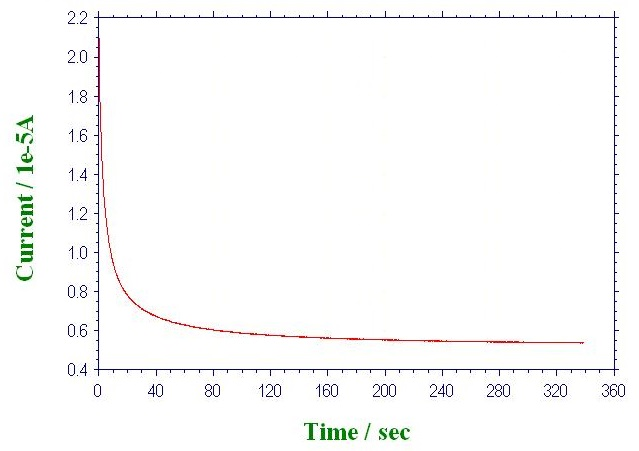
\includegraphics[width= \textwidth]{it25mV}

  \label{}
\end{subfigure}%
\begin{subfigure}{.5\textwidth}
  \centering
  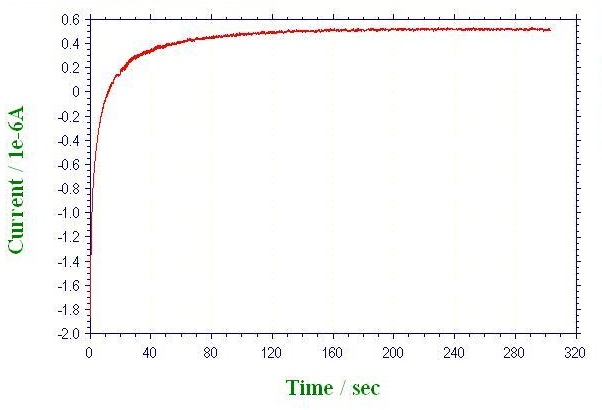
\includegraphics[width=.95 \linewidth]{it100mV}
  \label{}
\end{subfigure}
\caption{The amperometric i-t curve.  Right: the i-t curve of reducing conditions (-25 mV applied in this case). Left: the I-t curve of oxidizing conditions (100 mV applied in this case).}
\label{it_curves}
\end{figure}


\section*{Time trace analysis}
The software used for the fluorescence lifetime imaging and correlation software is SymPhoTime 64. With the help of this program, timetraces and its specific parameters are saved in .pt3 files. Older versions of SymPhoTime saved this data into .t3r files. Previous PhD student .. had written a program in MATLAB R2012b and C++ to read out the .t3r files and transfer the timetraces into multiple .dat files. This program has been adjusted in such a way it can read out the .pt3 files from the newer version of SymPhoTime 64. It allows you to manually select parts of the timetrace, as is shown in Figure \ref{timetrace_selection}.

\begin{figure}[ht!]
\centering
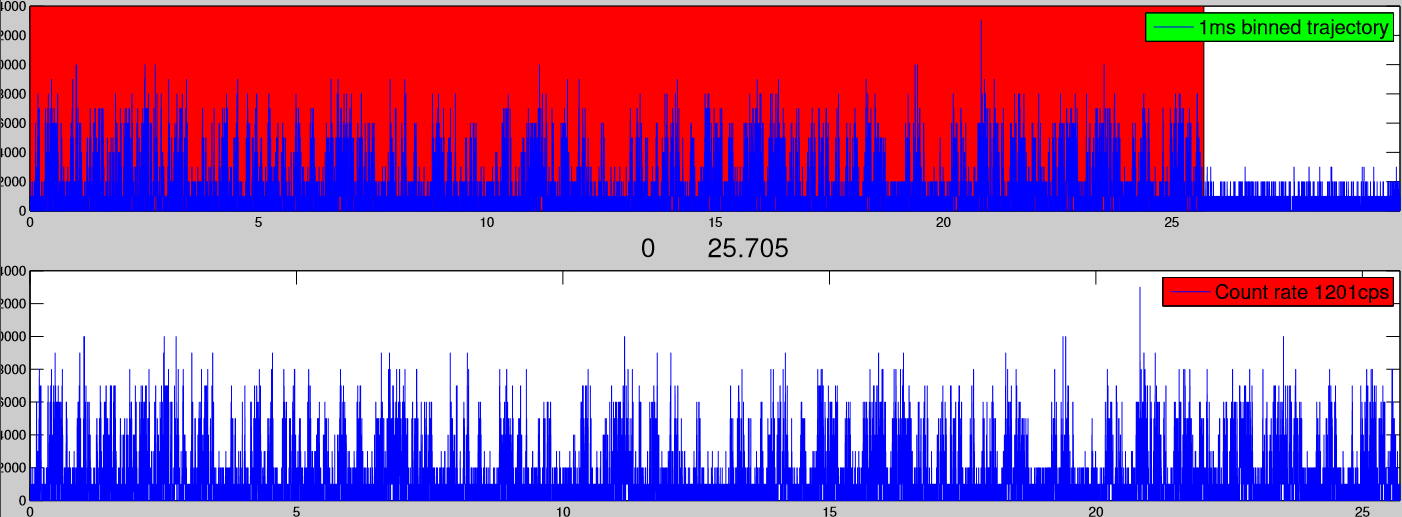
\includegraphics[width=\textwidth]{timetrace_selection}
\caption{Selection of a timetrace with a program written in MATLAB R2012b and C to select the parts of the timetrace (in red) that will be put into .dat files. As in this specific case the Cu-Azurin bleached around 25.7 second mark and the timetrace once it is bleached is not of interest and therefore not selected.}
\label{timetrace_selection}
\end{figure}

Once the timetrace is selected and put into several .dat files, another C program is run to precisely calculate the  on- ($\tau_{on}$) and off times ($\tau_{off}$). This program uses several mathematical methods to calculate the timestamps and intensity of intensity jumps in optical single molecule emission data that exhibit discrete intensity jumps, in detail described by Lucas P. Watkins and Haw Yang in their paper \cite{And2004}. As an example, several on- and off times are visualized in Figure \ref{on_off_times}. These times are defined as the duration of the CuAz being oxidized ($\tau_{on}$) and reduced ($\tau_{off}$). The intensity jumps that are controlled is what is referred to as 'switching' while the (often) unwanted and uncontrolled switching between the bright 'on' and dark 'off' states is called 'blinking'. 

\subsection*{Results and discussion timetraces CuAz}

Looking at the timetraces between 100mV and 0mV (Figure \ref{plots_timetraces_diff_pot}) a trend is noticeable on sight. For the higher potentials, the $\tau_{off}$ are long and the $\tau_{on}$ are relatively short which goes hand in hand with the low amount of events. When the potential decreases the amount of events start to increase and the $\tau_{on}$ becomes longer while $\tau_{off}$ becomes shorter. The explanation for this is simply the FluRedox principle. CuAz in oxidized form (copper is in $\textup{Cu}^{2+}$) shows an absorbence maximum around 628nm which overlaps with the fluorescence emission of the ATTO655 dye as is shown earlier in Figure \ref{}. Since FRET is high in this form, the fluorescence of the dye is quenched resulting in longer $\tau_{off}$. When the potential is decreasing, the solution is reducing. When CuAz is reduced - since the absorption at 628nm disappears upon reduction - the FRET is low and thus the dye  shows high fluorescence and longer $\tau_{on}$ times are expected. This principle seems to be the only role in play until the potential comes near 25mV. Here a new phenomenon is noticeable. Beside the expected  increasing $\tau_{on}$ and decreasing $\tau_{off}$ due to switching of CuAz, a secondary timescale seems to be shown in the form of very short $\tau_{on}$ in very short succession. To explain this event, a closer look has to be taken at the chemicals involved in the chemical processes concerning the redox reactions. Apart from the intramolecular electron transfer between the label and the copper center, intermolecular reactions between the redox active components in the solution and the dye are also present. For higher potentials, the time scale of the events between dye and solution are relatively high. When the potential gets lower, the solution is more and more reduced. The interaction between the dye and the reduced ascorbate and ferricyanide happen on a smaller timescale and is now prominent in the timetraces. This is more apparent when looked at the autocorrelation. The probability $I(t)$ of emission of a photon by an excited state at time t is determined by
\begin{equation} \label{solt}
dI(t) = -\frac{1}{\tau(t)}I(t)dt.
\end{equation}
The solution of equation \ref{solt} in the case of $\tau(t) = \tau_{0}= constant$ is the classical single exponential decay function. At higher potentials the autocorrelation can be fitted with this single exponential in the form of
\begin{equation} \label{single_exp}
g(\tau) =  A_{1}e^{-\tau/t_{1}}
\end{equation}
where $t_{1}$ and $A_{1}$ are constants. These constants are related to the on- and offtimes via the equations
\begin{equation}\label{tau_on}
\tau_{on} = t_{1} +\frac{t_{1}}{A_{1}}
\end{equation}
and
\begin{equation}\label{tau_off}
\tau_{off} = t_{1} +t_{1}A_{1}.
\end{equation}
When the potential is lowered towards the 25 mV and below, a single potential does not fit the autocorrelation but rather a sum of two exponentials fits the autocorrelation: 
\begin{equation}\label{multi_exp}
g(\tau) = A_{1}e^{-\tau/t_{1}} + A_{2}e^{-\tau/t_{2}}. 
\end{equation}
The constant-pair $t_{1}$ and $A_{1}$ and $t_{2}$ and $A_{2}$ are related with the on- and off-times according equation \ref{tau_on} and equation \ref{tau_off}. The longer $\tau_{on}$ are the ones from the switching of the CuAz, while the shorter $\tau_{on}$ is the one due to the blinking of the dye.


\begin{figure}[ht!]
\centering
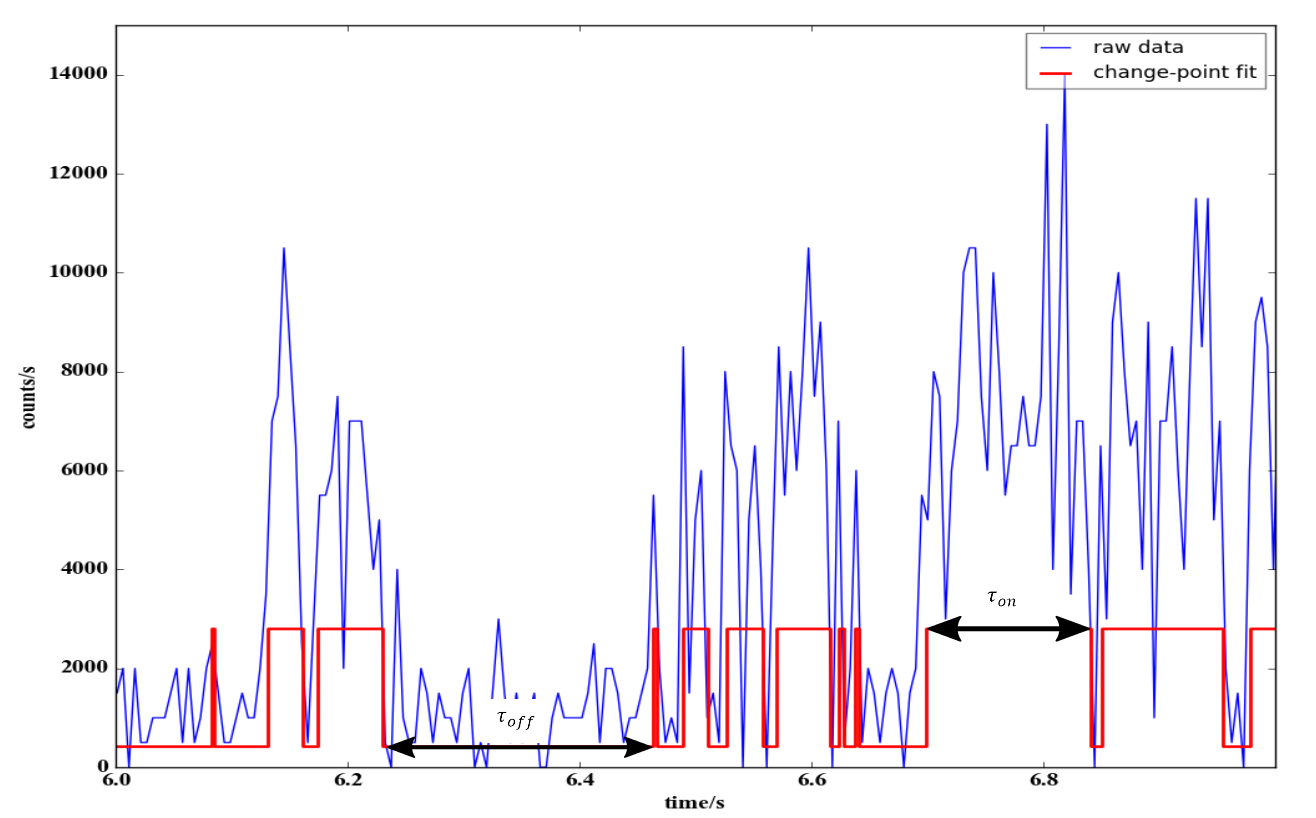
\includegraphics[width=\textwidth]{on_off_test1}
\caption{Same timetrace as Figure \ref{timetrace_selection} but a smaller range. In red is plotted the calculated intensity jumps according to the program written by Lucas P. Watkins and Haw Yang. The time when the intensity is low is referred to as the $\tau_{off}$ and the time the molecules intensity is high is the $\tau_{on}$.}
\label{on_off_times}
\end{figure}

\begin{figure}[ht!]
\centering
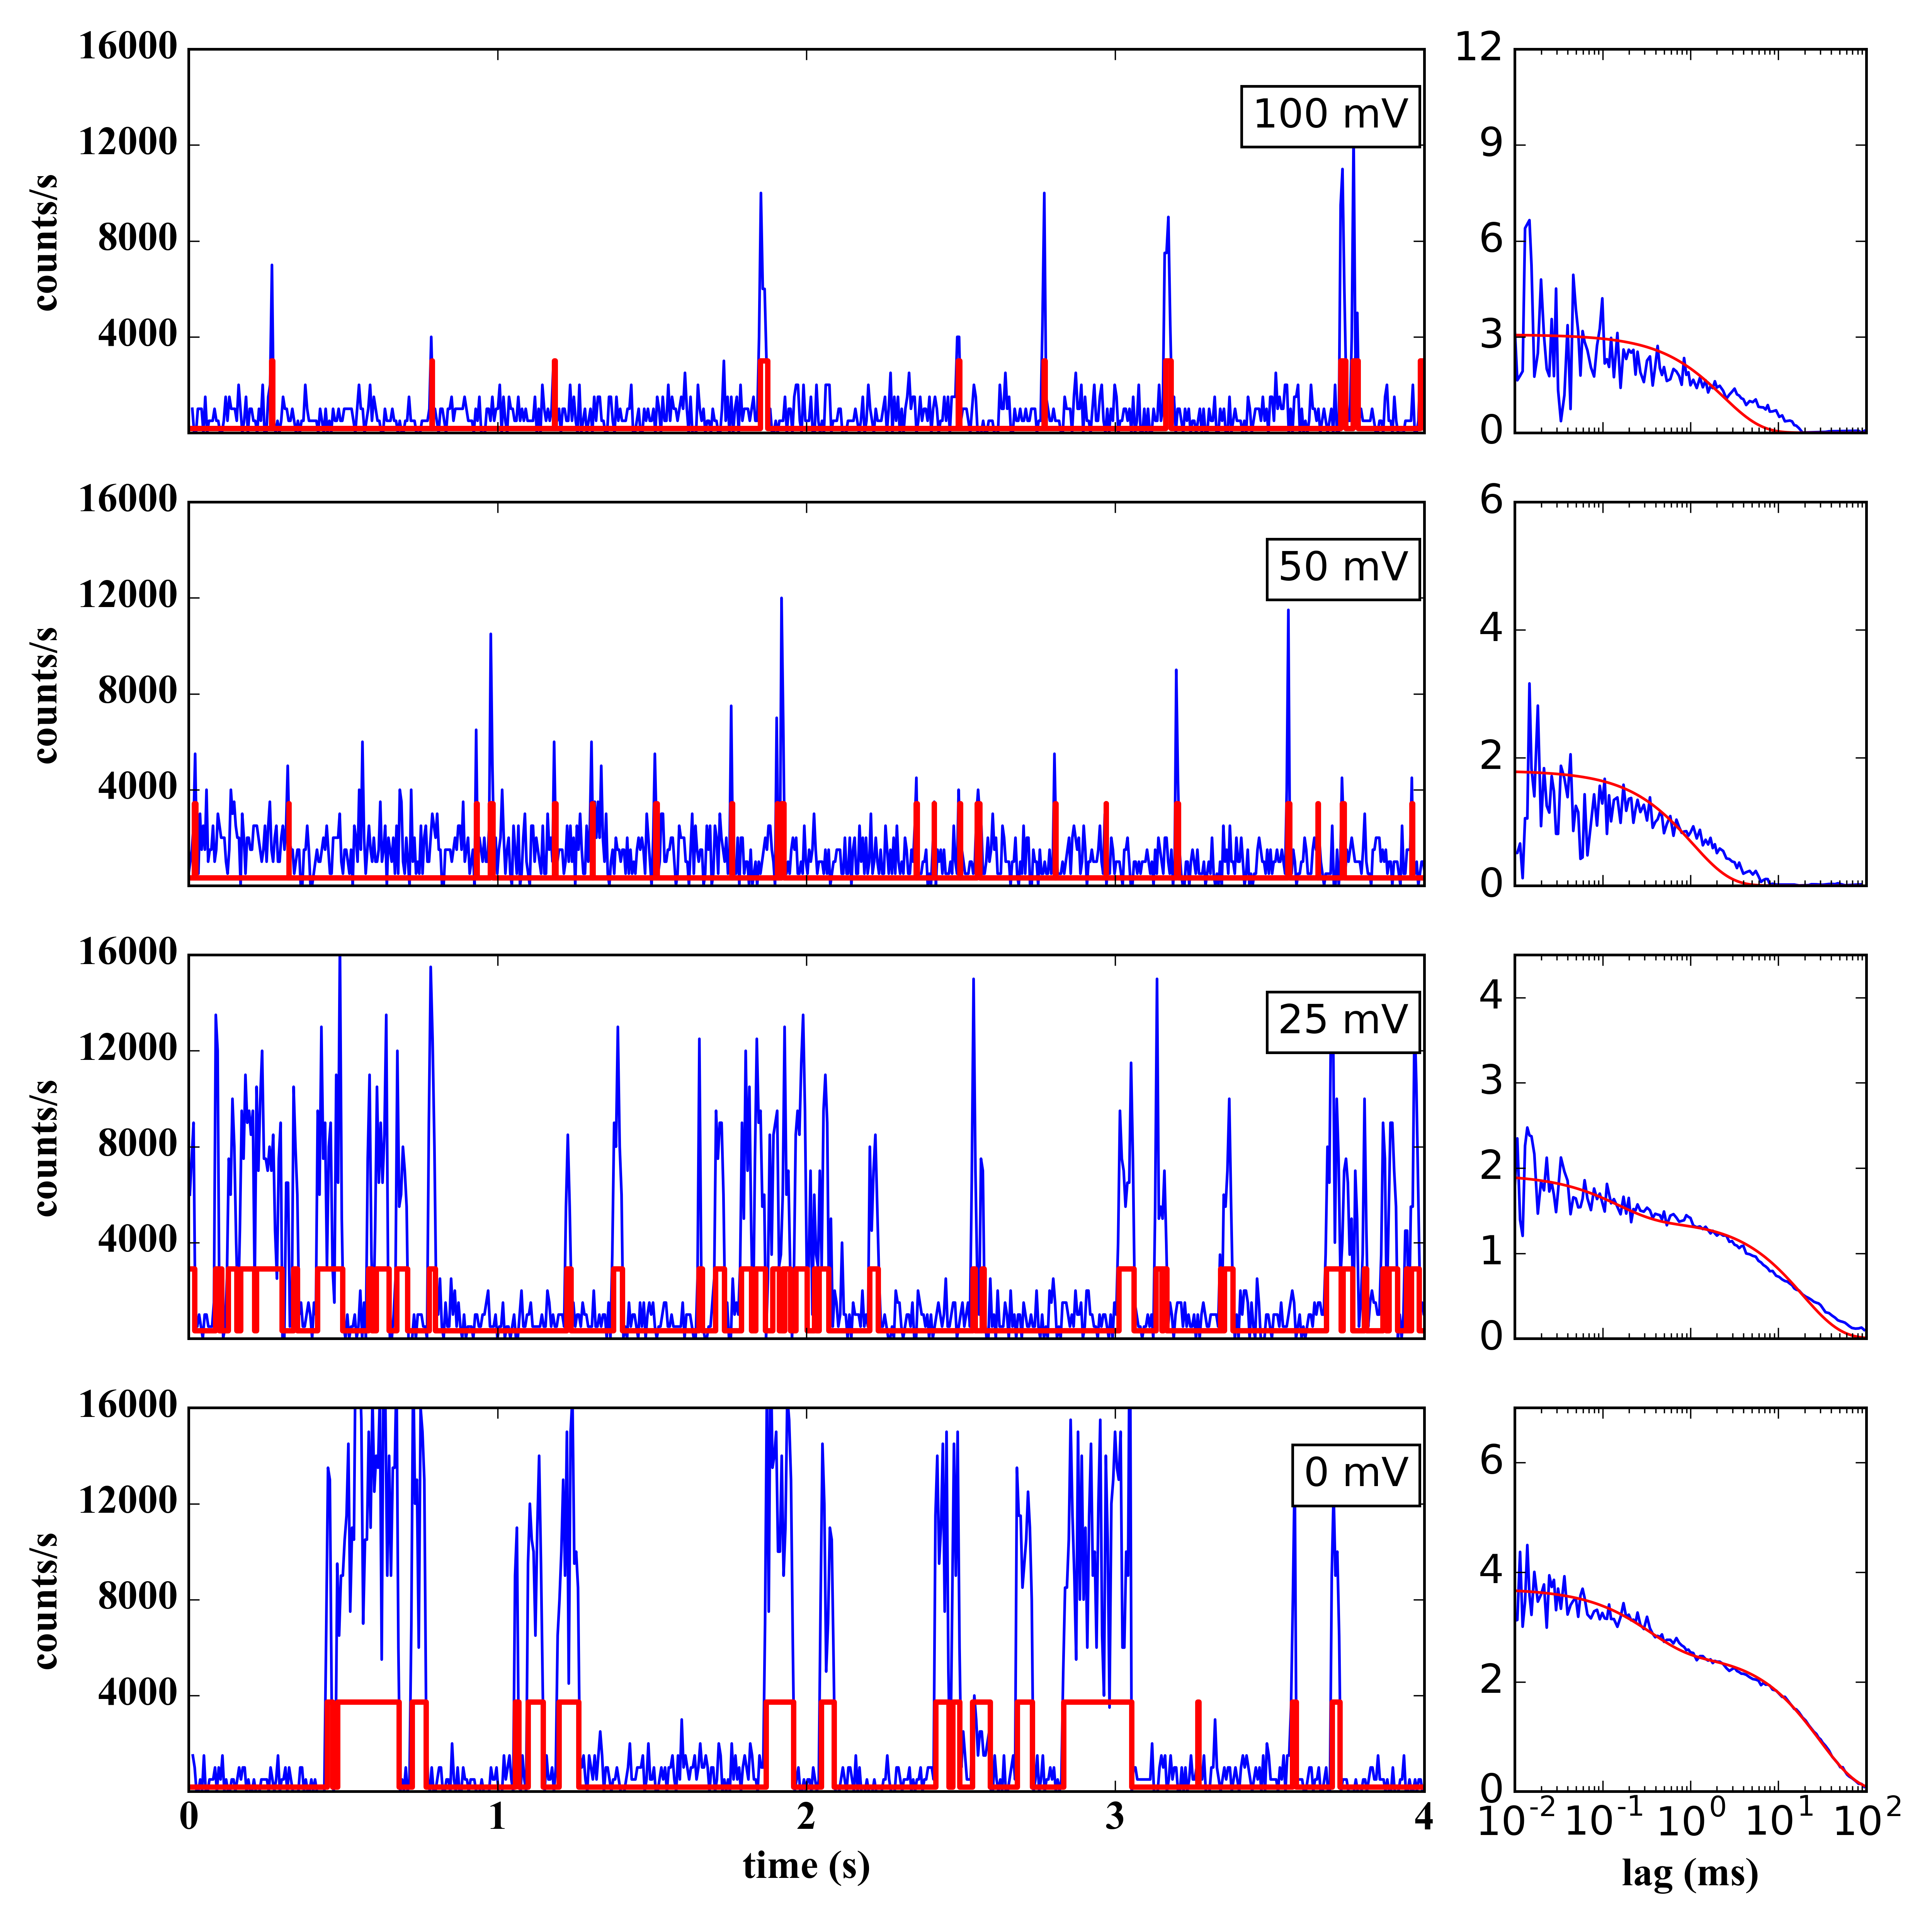
\includegraphics[width=1\textwidth]{plots_timetraces_diff_pot}
\caption{Timetraces together with its autocorrelation of the same CuAz molecule under different potentials. A clear difference between $\tau_{on}$ and $\tau_{on}$ under different potentials is visible: shorter $\tau_{on}$ for higher oxidizing potentials, longer $\tau_{on}$ for reducing lower potentials. For potentials below 25mV this pattern gets disturbed due to blinking of the ATTO665. This phenomenon is shown in the autocorrelation by changing from a single exponential fit to a multi-exponential fit.}
\label{plots_timetraces_diff_pot}
\end{figure}



Another way of looking at the $\tau_{on}$ and  $\tau_{off}$ is by plotting the distribution of the on and off times in the time traces. This is done in Figure \ref{histograms_disc}. The fit through these histograms will give the average on- and off-times. A very interesting phenomenon is observed in the off-times however. Where the on-times are fitted with a single exponent, the off-times have a different form. Very short off-times seem to be relatively rare. To get a deeper understanding of this a closer look has to be taken at the electron transfer process between the solution and the copper azurin.
\begin{equation}\label{ox_pros}
\textup{Cu}^{2+}\xleftarrow[3]{\overset{1}{\longrightarrow}\textup{Cu}^{2+}+ e^{-}\overset{2}{\longrightarrow}}\textup{Cu}^{1+}
\end{equation}
The reduction of $\textup{Cu}^{2+}$ to $\textup{Cu}^{1+}$ is a multi-step process. Bringing the electron close to the copper center (step 1) and reducing the copper (step 2) is happening in two short time scales. Contrary to the reduction of copper azurin, the oxidation is a single step process. This should go faster than reducing and thus shorter off times are expected to be much more present. This is in contradiction to the histograms which show an absence of these short times. Something in step 3 is delaying the oxidation. With the model presented above, this cannot be explained and further research to this subject is needed.

\begin{figure}[ht!]
\centering
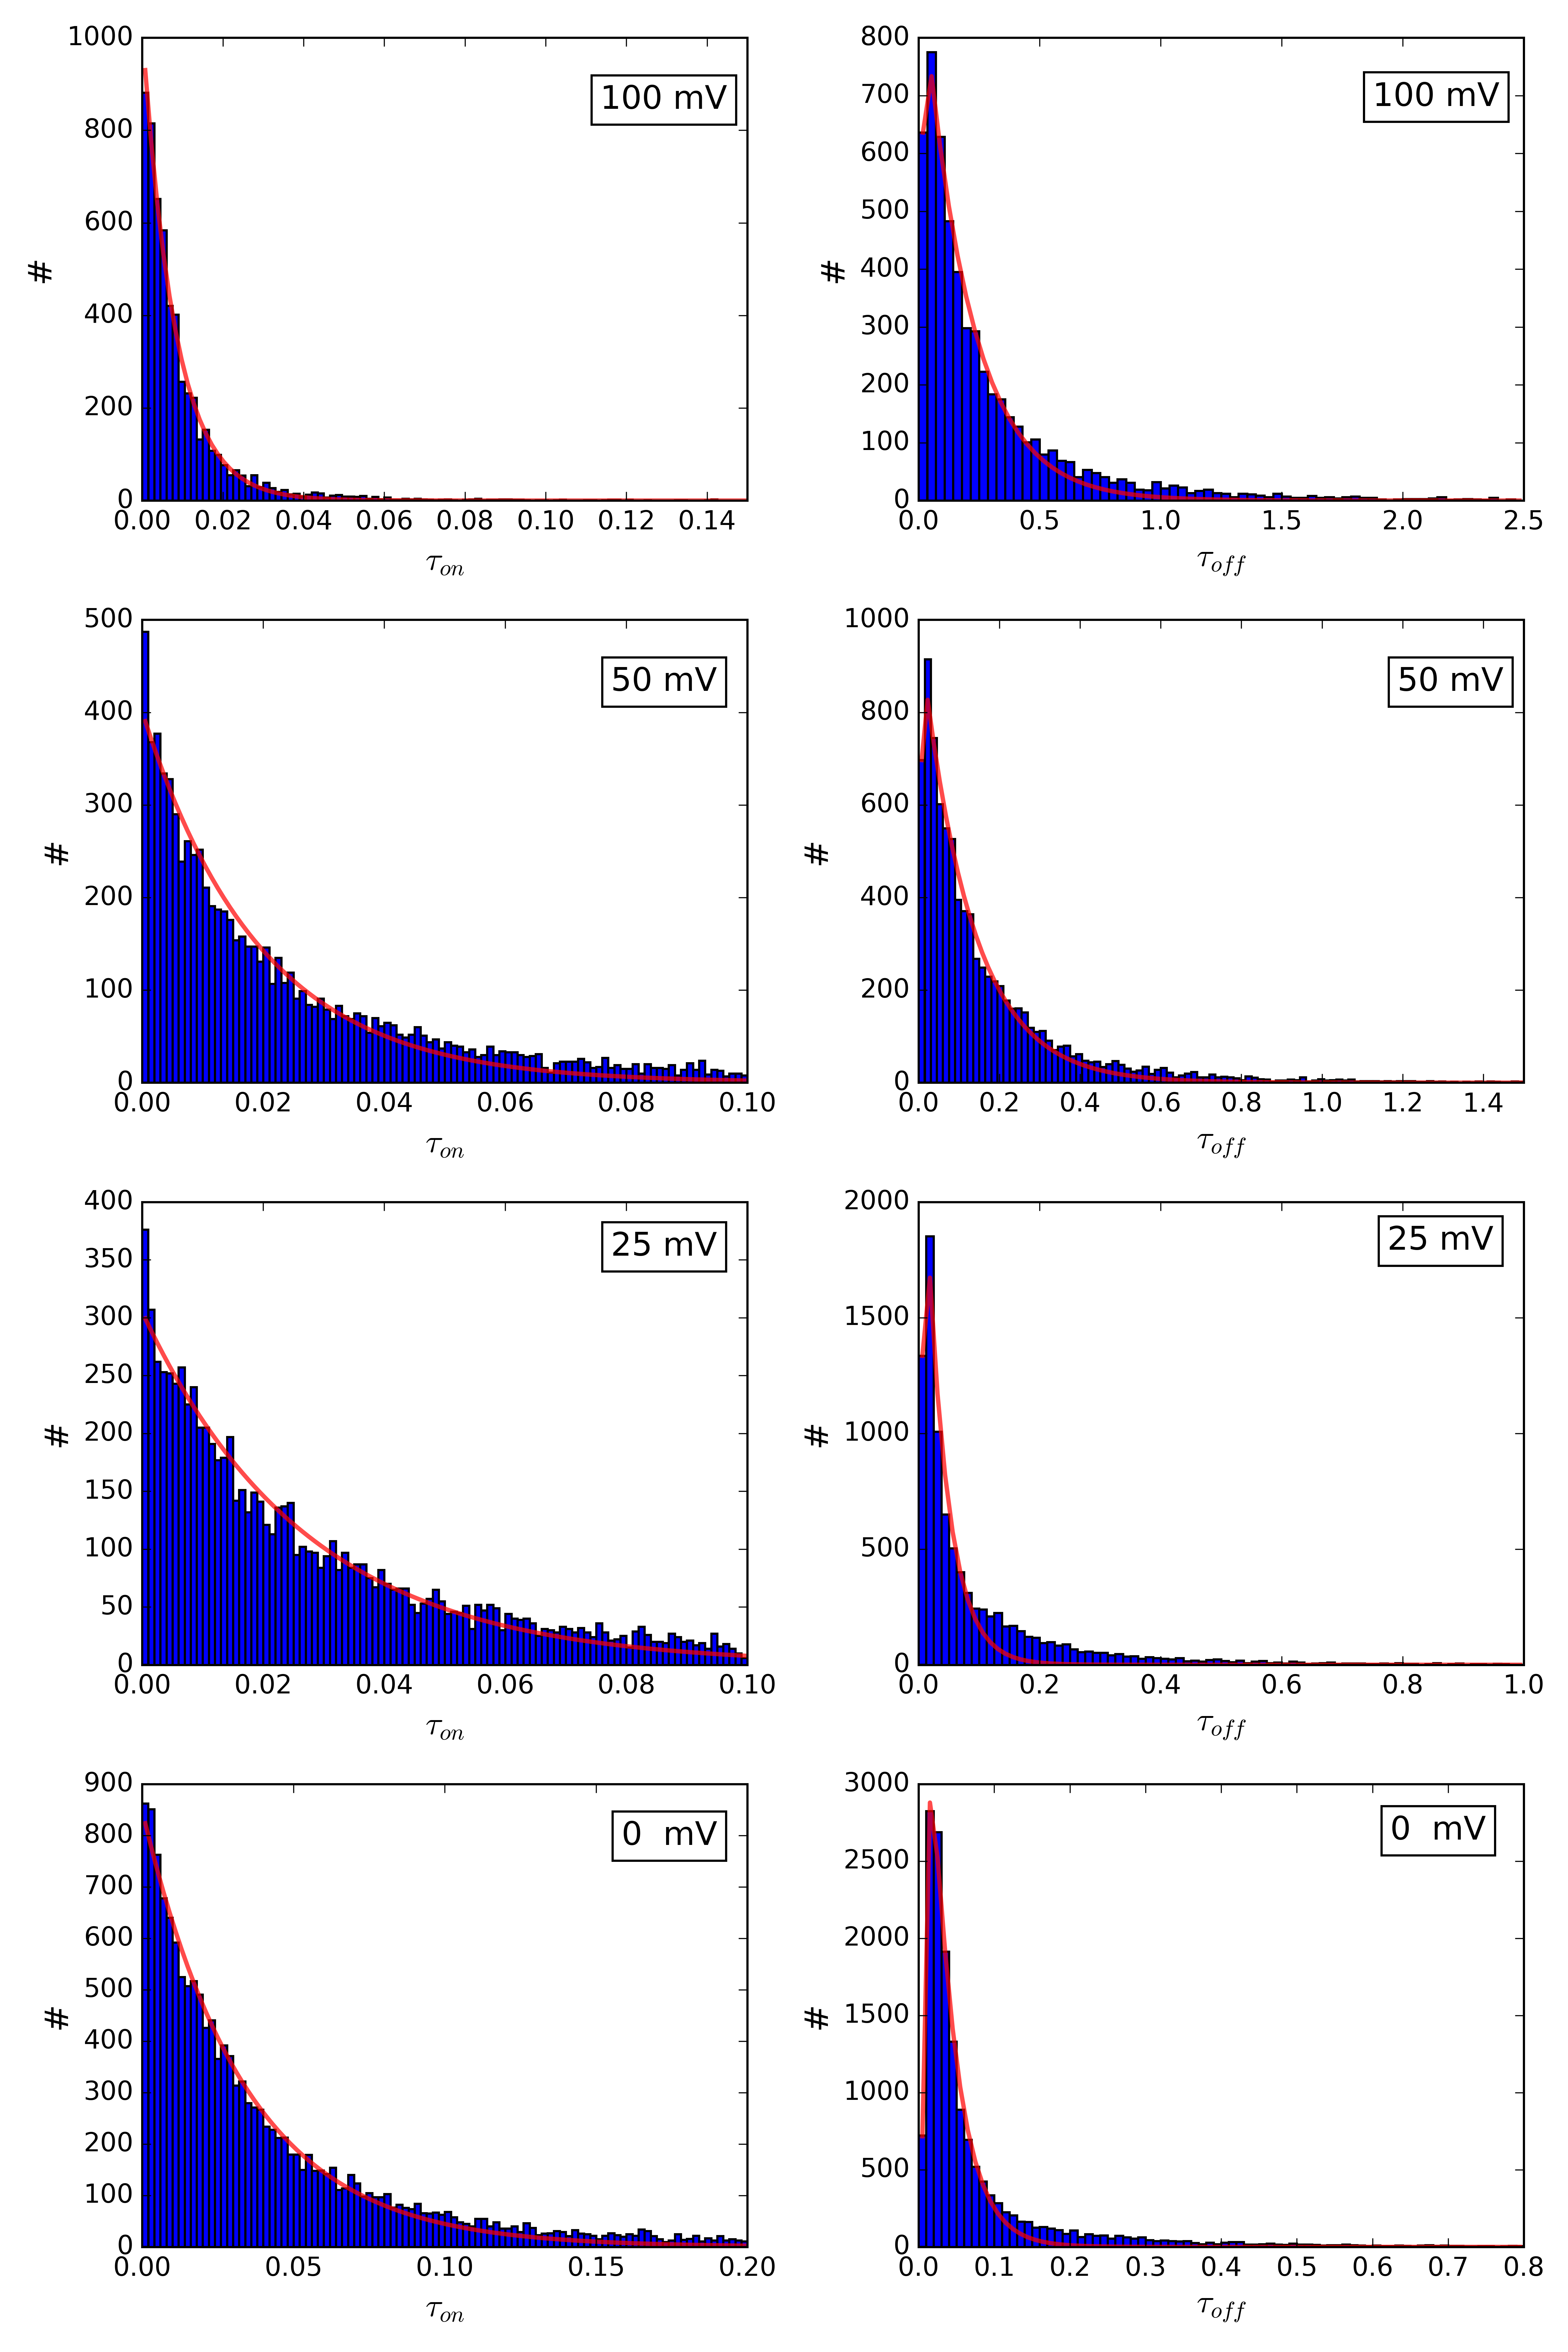
\includegraphics[width=.9\textwidth]{histograms_thesis}
\caption{Histogram distribution $\tau_{on}$ and $\tau_{off}$ at different potentials.}
\label{histograms_disc}
\end{figure}

To give the switching of the CuAz a more quantitatively meaning, the average $\tau_{on}$ ($\bar{\tau}_{on}$) and average $\tau_{on}$ ($\bar{\tau}_{off}$) can be related to the Nernst equation since the switching is due to the redox reaction of CuAz. Rewriting equation \ref{nernst} to 

\begin{equation}\label{nernst_tau}
E = E_{0}+\frac{k_{B}T}{ne}\textup{ln}\frac{\bar{\tau}_{off}}{\bar{\tau}_{on}}
\end{equation}
the average on- and off-times can be related to the potential applied. Rewriting equation \ref{nernst_tau} leads to
\begin{equation}\label{fit_onoff}
\frac{\bar{\tau}_{off}}{\bar{\tau}_{on}} = \textup{exp}\left ( \frac{E_{0}-E}{0.059} \right ).
\end{equation}
A fit through the ratio of the $\frac{\bar{\tau}_{off}}{\bar{\tau}_{on}}$ and the applied potential $E$ will lead to the midpoint potential $E_{0}$ of the protein. The on- and off-times above 30 mV are extracted directly from the time traces. For the potentials below 30 mV, the on- and off-times are extracted from the autocorrelation. Since the fit for the autocorrelation consist of two exponentials, the exponent in which the $\tau_{on}$ has the smallest value is considered to be the one belonging to the blinking of the dye. Using this rule the ratio $\frac{\bar{\tau}_{off}}{\bar{\tau}_{on}}$ that belongs to the CuAz can be determined for values below the 30 mV. Using the data of one experimental day: 19 different protein under at least 8 different potentials between 0 mV and 100 mV, the midpoint potential is determined to be 25.62 mV. This is in accordance with the 25 mV given in other literature (citation needed). 

\begin{figure}[ht!]
\centering
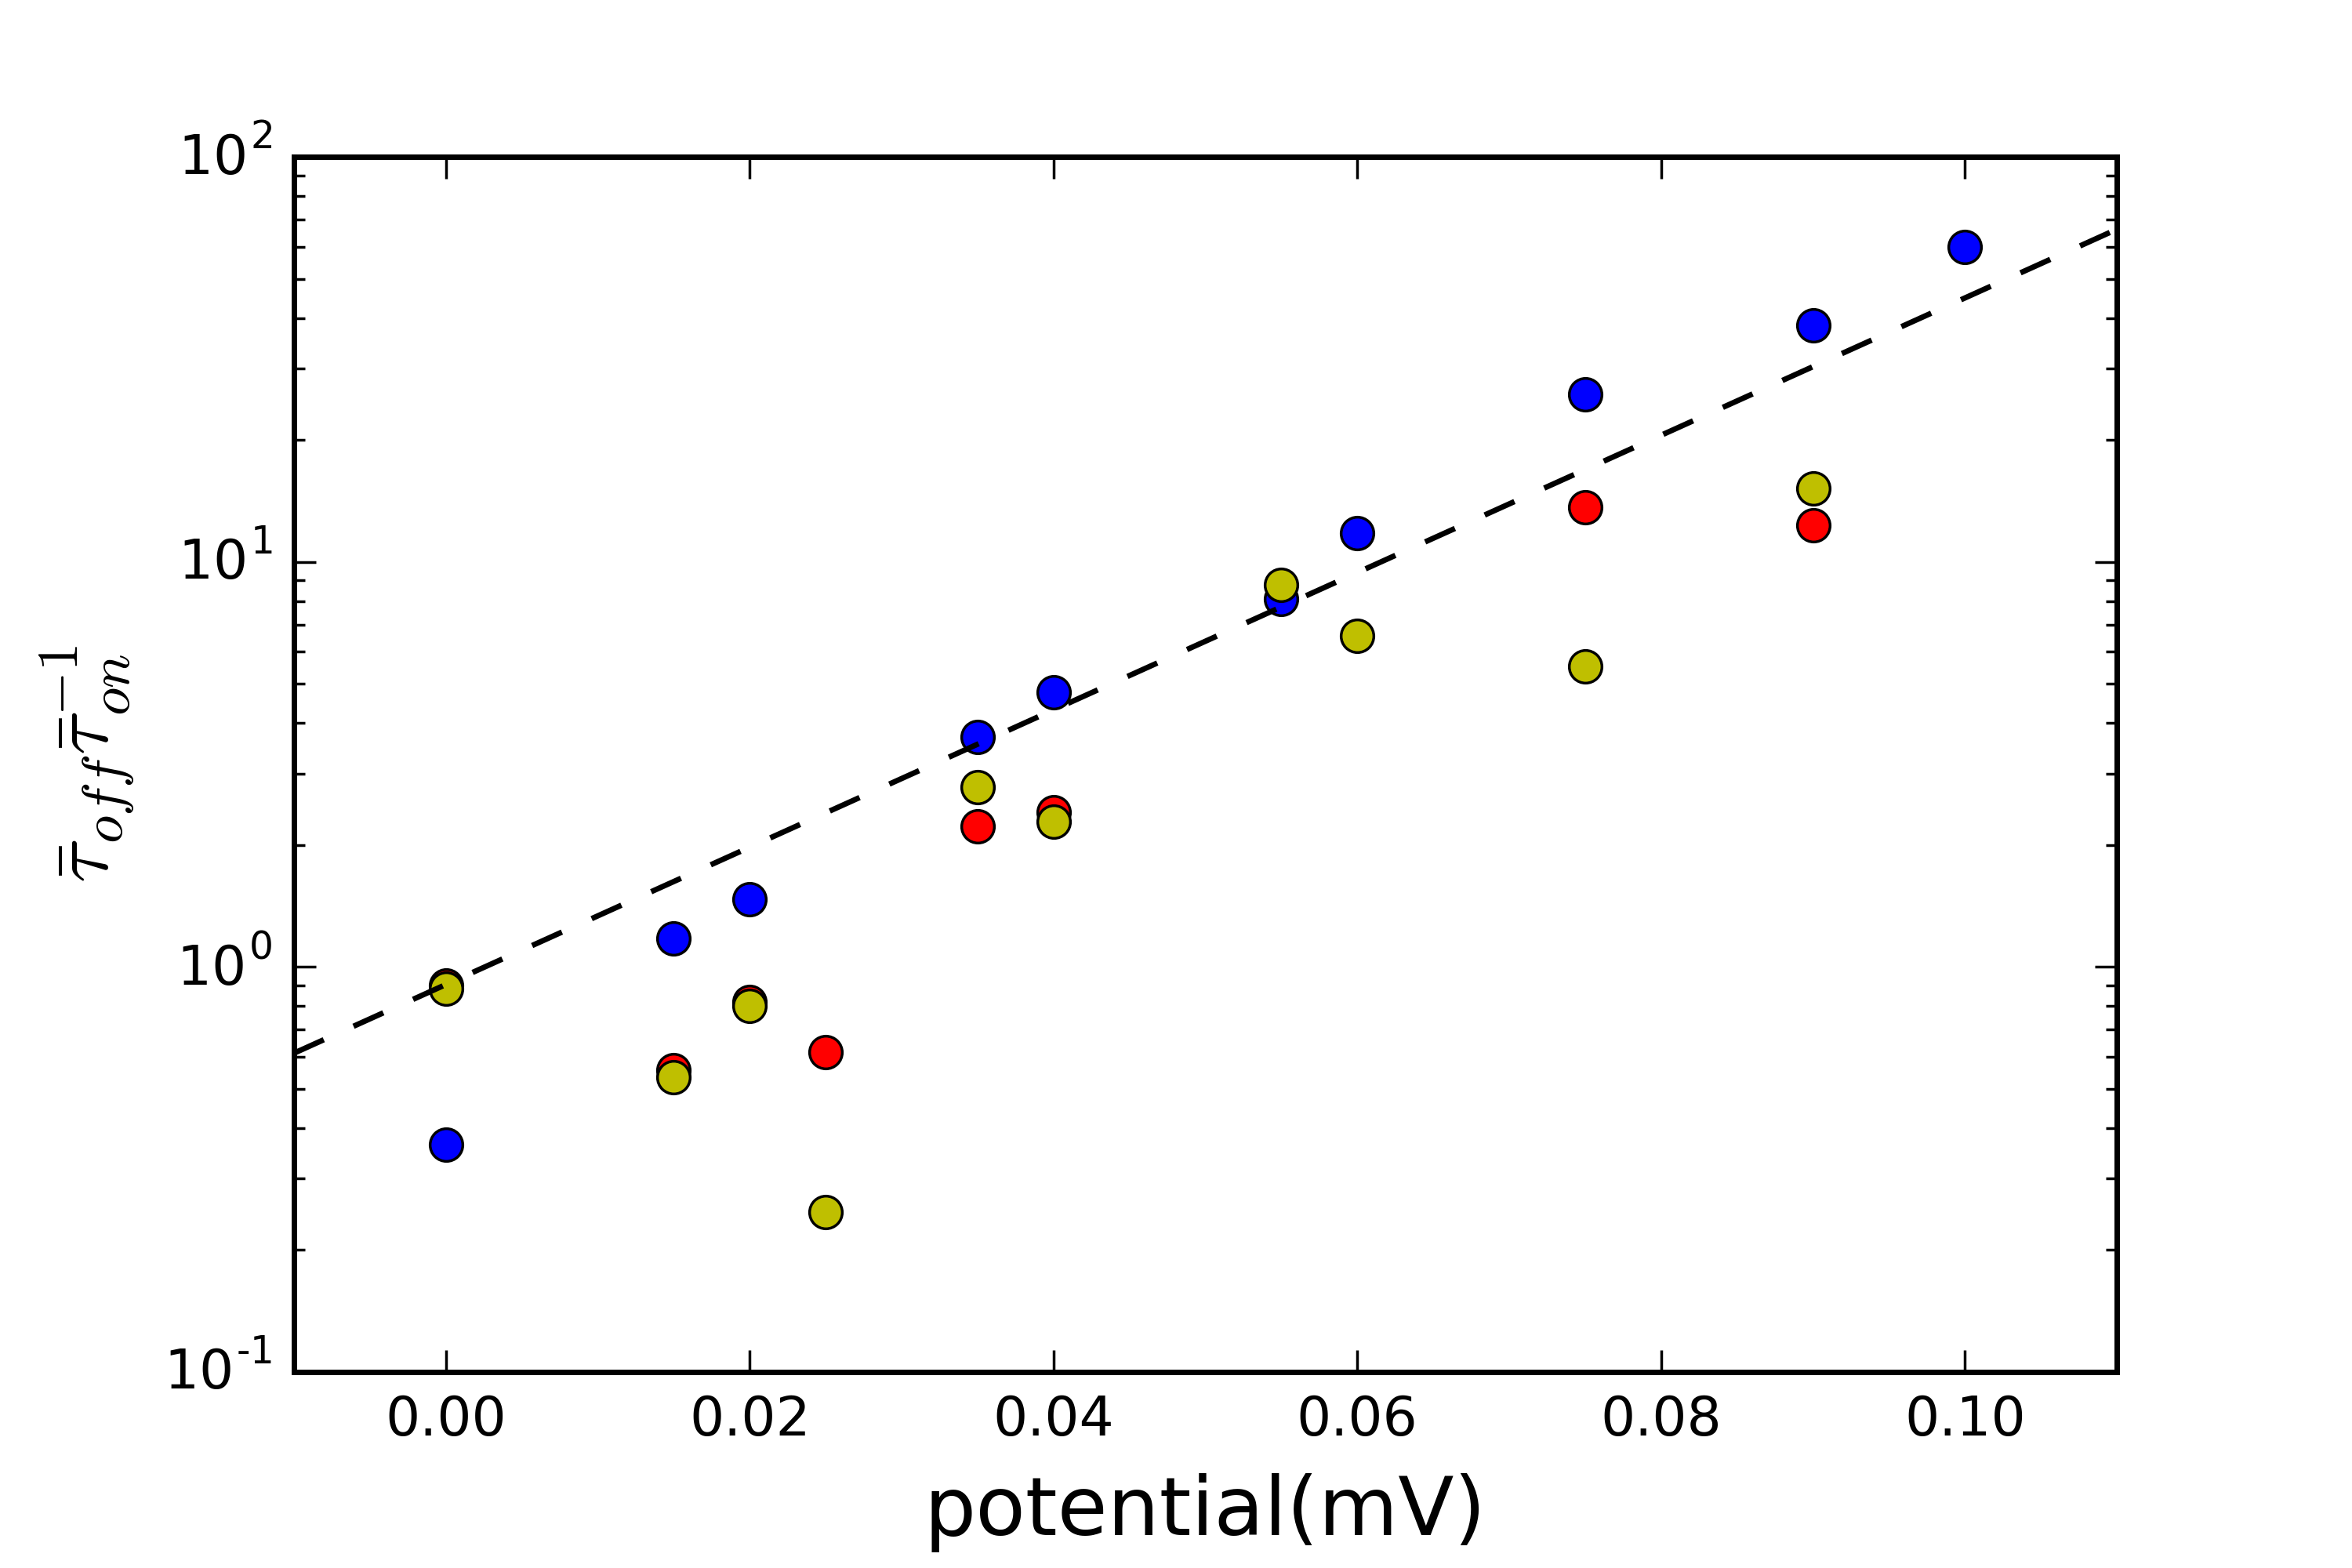
\includegraphics[width=.9\textwidth]{t_ratio_plot}
\caption{Plot of the ratio of $\frac{\bar{\tau}_{off}}{\bar{\tau}_{on}}$ versus the potential of three different CuAz proteins (each represented with a different color). The dashed black line is the average fit of 15 different single CuAz.}
\label{t_ratio_plot}
\end{figure}


\end{document}
